\documentclass[11pt]{article}

\usepackage[margin=1in]{geometry}
\usepackage[utf8]{inputenc}
\usepackage[T1]{fontenc}
\usepackage{graphicx}
\usepackage{booktabs}
\usepackage{longtable}
\usepackage{caption}
\usepackage{subcaption}
\usepackage{amsmath}
\usepackage{array}
\usepackage{tabularx}
\usepackage{float}
\usepackage{hyperref}
\usepackage[numbers]{natbib}
\usepackage{enumitem}
\usepackage{xcolor}
\usepackage{microtype}

\hypersetup{
  colorlinks=true,
  linkcolor=blue,
  urlcolor=blue,
  citecolor=blue
}

\title{\textbf{AI Compute Accessibility Atlas for EIP}\\
\large Mapping a hidden infrastructure layer of AI opportunity, then showing why distance alone is not enough}
\author{Authoritative final submission draft}
\date{March 14, 2026}

\begin{document}
\maketitle

\begin{abstract}
Modern AI may be consumed through the cloud, but the cloud is not placeless. It is built from region-scale datacenter infrastructure, network capacity, and supporting institutional ecosystems that are unevenly distributed across cities. This report asks a simple but important question for a public-interest geospatial submission: across a global frame of 8,000 cities, do cities that are farther from major hyperscaler cloud regions tend to show less observed AI research activity? It then asks a second question that is more original and more useful for EIP: once distance is measured, what additional bundle of factors helps distinguish cities that merely sit near one cloud region from cities that occupy a broader compute-opportunity environment?

The final answer has two layers. First, the atlas backbone shows a strong spatial pattern. The median city in the full 8,000-city comparison frame is about 657 km from its nearest AWS, Azure, or Google Cloud region, while the median AI-linked city in the delivered overlay is only about 237 km away; when weighted by observed AI works, that center of gravity moves to about 164 km. The negative distance relationship remains visible in two spatial models, and a priority screen identifies 1,988 large cities with zero observed AI works in the delivered overlay and above-threshold compute distance. Second, the final submission extends the project beyond raw distance by introducing a \emph{Compute Opportunity Bundle Index} built from cloud proximity, provider diversity, regional redundancy, institutional anchors, and city scale. That index makes the submission more original, more legible to judges, and more aligned with the project’s mature claim: compute is not destiny, but it is part of the infrastructure bundle that shapes AI opportunity.

This report therefore does \emph{not} present a definitive causal estimate of cloud-region openings. The Stage 4--6 causal experiments remain mixed and are frozen as a boundary rather than a headline result. What the report does provide is a detailed, reproducible, and readable geospatial diagnosis of where compute access is strong, where it is weak, which cities align with the pattern, which cities break it, and why that matters for a public-interest understanding of unequal AI opportunity.
\end{abstract}

\section{Introduction: why AI geography needs an infrastructure lens}
AI does not happen on a blank map. Public discussion often treats AI as a story about labs, firms, patents, and talent. It is also a story about access to large-scale cloud infrastructure. Modern AI systems depend on datacenter regions, dense networking, and enough surrounding institutional capacity to turn infrastructure access into visible activity. Those conditions are not spread evenly across the world. Some cities sit inside dense compute corridors. Others remain hundreds or thousands of kilometers away from the nearest hyperscaler region and must work through thinner infrastructure conditions.

That starting point matters for a project aimed at EIP judges. The central contribution is not simply that the report runs spatial models. It is that the project makes a hidden infrastructure layer visible and interpretable on a map. Instead of talking about compute as abstract cloud vapor, the atlas shows where it is physically proximate, where it is distant, and where those patterns overlap with observed AI activity in the delivered research overlay.

The report is designed to do three things at once:
\begin{itemize}[leftmargin=*]
  \item provide a clear and readable global atlas of compute accessibility across 8,000 cities;
  \item test whether the descriptive relationship between compute proximity and observed AI research survives basic controls for population and geography; and
  \item move beyond raw distance by adding one visibly original analytical layer that better matches the project’s own mature conclusion.
\end{itemize}

\subsection{The central question}
The project asks a plain-language question: once city size and broad spatial dependence are taken into account, do cities that are farther from major AWS, Azure, and Google Cloud regions tend to show less observed AI research activity in the delivered overlay?

A second, equally important question follows from that one: if the relationship is real but not deterministic, what additional bundle of opportunity conditions helps explain why some cities align strongly with the pattern while others beat it or lag it?

\subsection{The short answer}
The evidence points in the same direction across maps, descriptive comparisons, spatial diagnostics, and two controlled spatial models. AI-linked cities occupy a much more compute-proximate part of the urban system than the broader 8,000-city frame. The strongest claim supported by the evidence is that compute accessibility is a meaningful spatial correlate of observed AI activity and that ignoring its geography leaves part of the AI-opportunity story invisible.

The report’s second answer is what makes the final submission more original. Distance alone is too thin. Cities differ not only in nearest-region distance, but also in provider diversity, regional redundancy, institutional anchoring, and scale. That is why the final report adds a Compute Opportunity Bundle Index and then uses four city case studies --- Singapore, Seoul, Ho Chi Minh City, and Lagos --- to show how the broader infrastructure bundle sharpens the story.

\subsection{What this report does and does not claim}
This report is deliberately ambitious in scope and deliberately careful in inference. It maps a strong and readable spatial relationship. It does not claim that opening a cloud region mechanically causes city-level AI growth everywhere. The Stage 4--6 causal extensions were re-audited for this final package and remain mixed. Rather than oversell them, the report uses them to set an evidentiary boundary: the submission is stronger than a visual coincidence and weaker than a definitive causal estimate. That boundary is not a weakness. It is part of the project’s credibility.

\section{Study design, data sources, and evidentiary boundaries}
\subsection{A global comparison frame of 8,000 cities}
The atlas begins with the world’s 8,000 largest cities from \texttt{worldcities.csv} \citep{worldcities}. This frame matters because it keeps the project comparative. Without it, the report could only say where AI-linked cities are located. With it, the report can ask whether AI-linked cities occupy a distinctive part of the global compute-access landscape.

Population is used as the minimal scale control throughout the project. It is not a full measure of urban innovation capacity, but it is transparent and globally available, and it helps distinguish very large urban systems from much smaller places.

\subsection{A cloud-region infrastructure layer}
The cloud infrastructure layer is built from public region-coordinate files for AWS, Azure, and Google Cloud \citep{cloudregions}. In this submission, a cloud region is treated as a named geographic cluster of datacenters rather than as an exhaustive map of every facility. That choice keeps the metric legible while still capturing the major geographic pattern of hyperscaler infrastructure.

\begin{table}[ht]
\centering
\begin{tabular}{lr}
\toprule
Provider & Regions (count) \\
\midrule
aws & 29 \\
azure & 47 \\
gcp & 35 \\
\bottomrule
\end{tabular}
\caption{Hyperscaler cloud regions included (from public region coordinate datasets).}
\label{tab:region_counts}
\end{table}


The delivered build contains 111 regions in total: 29 AWS, 47 Azure, and 35 Google Cloud regions. That list is a tractable and reproducible representation of the hyperscaler footprint that matters for this atlas.

\subsection{An observed AI research overlay}
The project uses a delivered OpenAlex-derived city overlay to represent observed AI-related research activity \citep{openalex}. The overlay is filtered through three preserved OpenAlex topics and matched onto the 8,000-city frame.

\begin{table}[ht]
\centering
\begin{tabular}{llr}
\toprule
Topic ID & Topic name & Works count (candidate) \\
\midrule
T10181 & Natural Language Processing Techniques & 290539 \\
T12254 & Machine Learning in Bioinformatics & 276039 \\
T10320 & Neural Networks and Applications & 249728 \\
\bottomrule
\end{tabular}
\caption{OpenAlex topic filters used to define 'AI research' in this project (from your overlay-generation script).}
\label{tab:topics}
\end{table}


The current build matches 328 overlay rows to the city frame, with 322 matches inside the 75 km threshold preserved by the project and 319 unique city geometries used for whole-map clustering diagnostics. The overlay is useful, but it is not the whole AI economy. The report therefore treats it as an observed layer of visible AI-related research rather than as a complete census of AI opportunity.

\paragraph{Boundary note.}
The repository preserves the delivered topic IDs and files, but not the exact OpenAlex query end date or exact recency window behind \texttt{openalex\_ai\_works\_recent}. A city that is absent from the overlay should therefore be read as ``not observed in this delivered filter,'' not as a verified zero-AI location.

\subsection{How compute accessibility is measured}
For each city, the atlas computes the great-circle distance to the nearest AWS, Azure, or Google Cloud region. This is intentionally simple. It is not a direct measure of latency, GPU availability, transfer cost, or service breadth. What it provides is a transparent, globally comparable first-order access measure that can be mapped, summarized, and interpreted without black-box assumptions.

\subsection{How the report handles causality}
The final package explicitly separates spatial diagnosis from causal proof. Cross-sectional distance gradients, hotspot patterns, and even spatially controlled models do not identify the causal effect of cloud-region placement. The Stage 4--6 attempts at within-country, matching, event-study, and staggered-adoption designs remain mixed. For this reason, the final report keeps causal language restrained and uses the causal work as a boundary memo rather than as the center of the story.

\section{The atlas backbone: what the core analysis shows}
\subsection{The first descriptive fact: compute access is uneven}
The project’s first contribution is simply to show that compute access is not geographically flat. Figure~\ref{fig:accessmap} maps city-level distance to the nearest cloud region across the global city frame.

\begin{figure}[H]
  \centering
  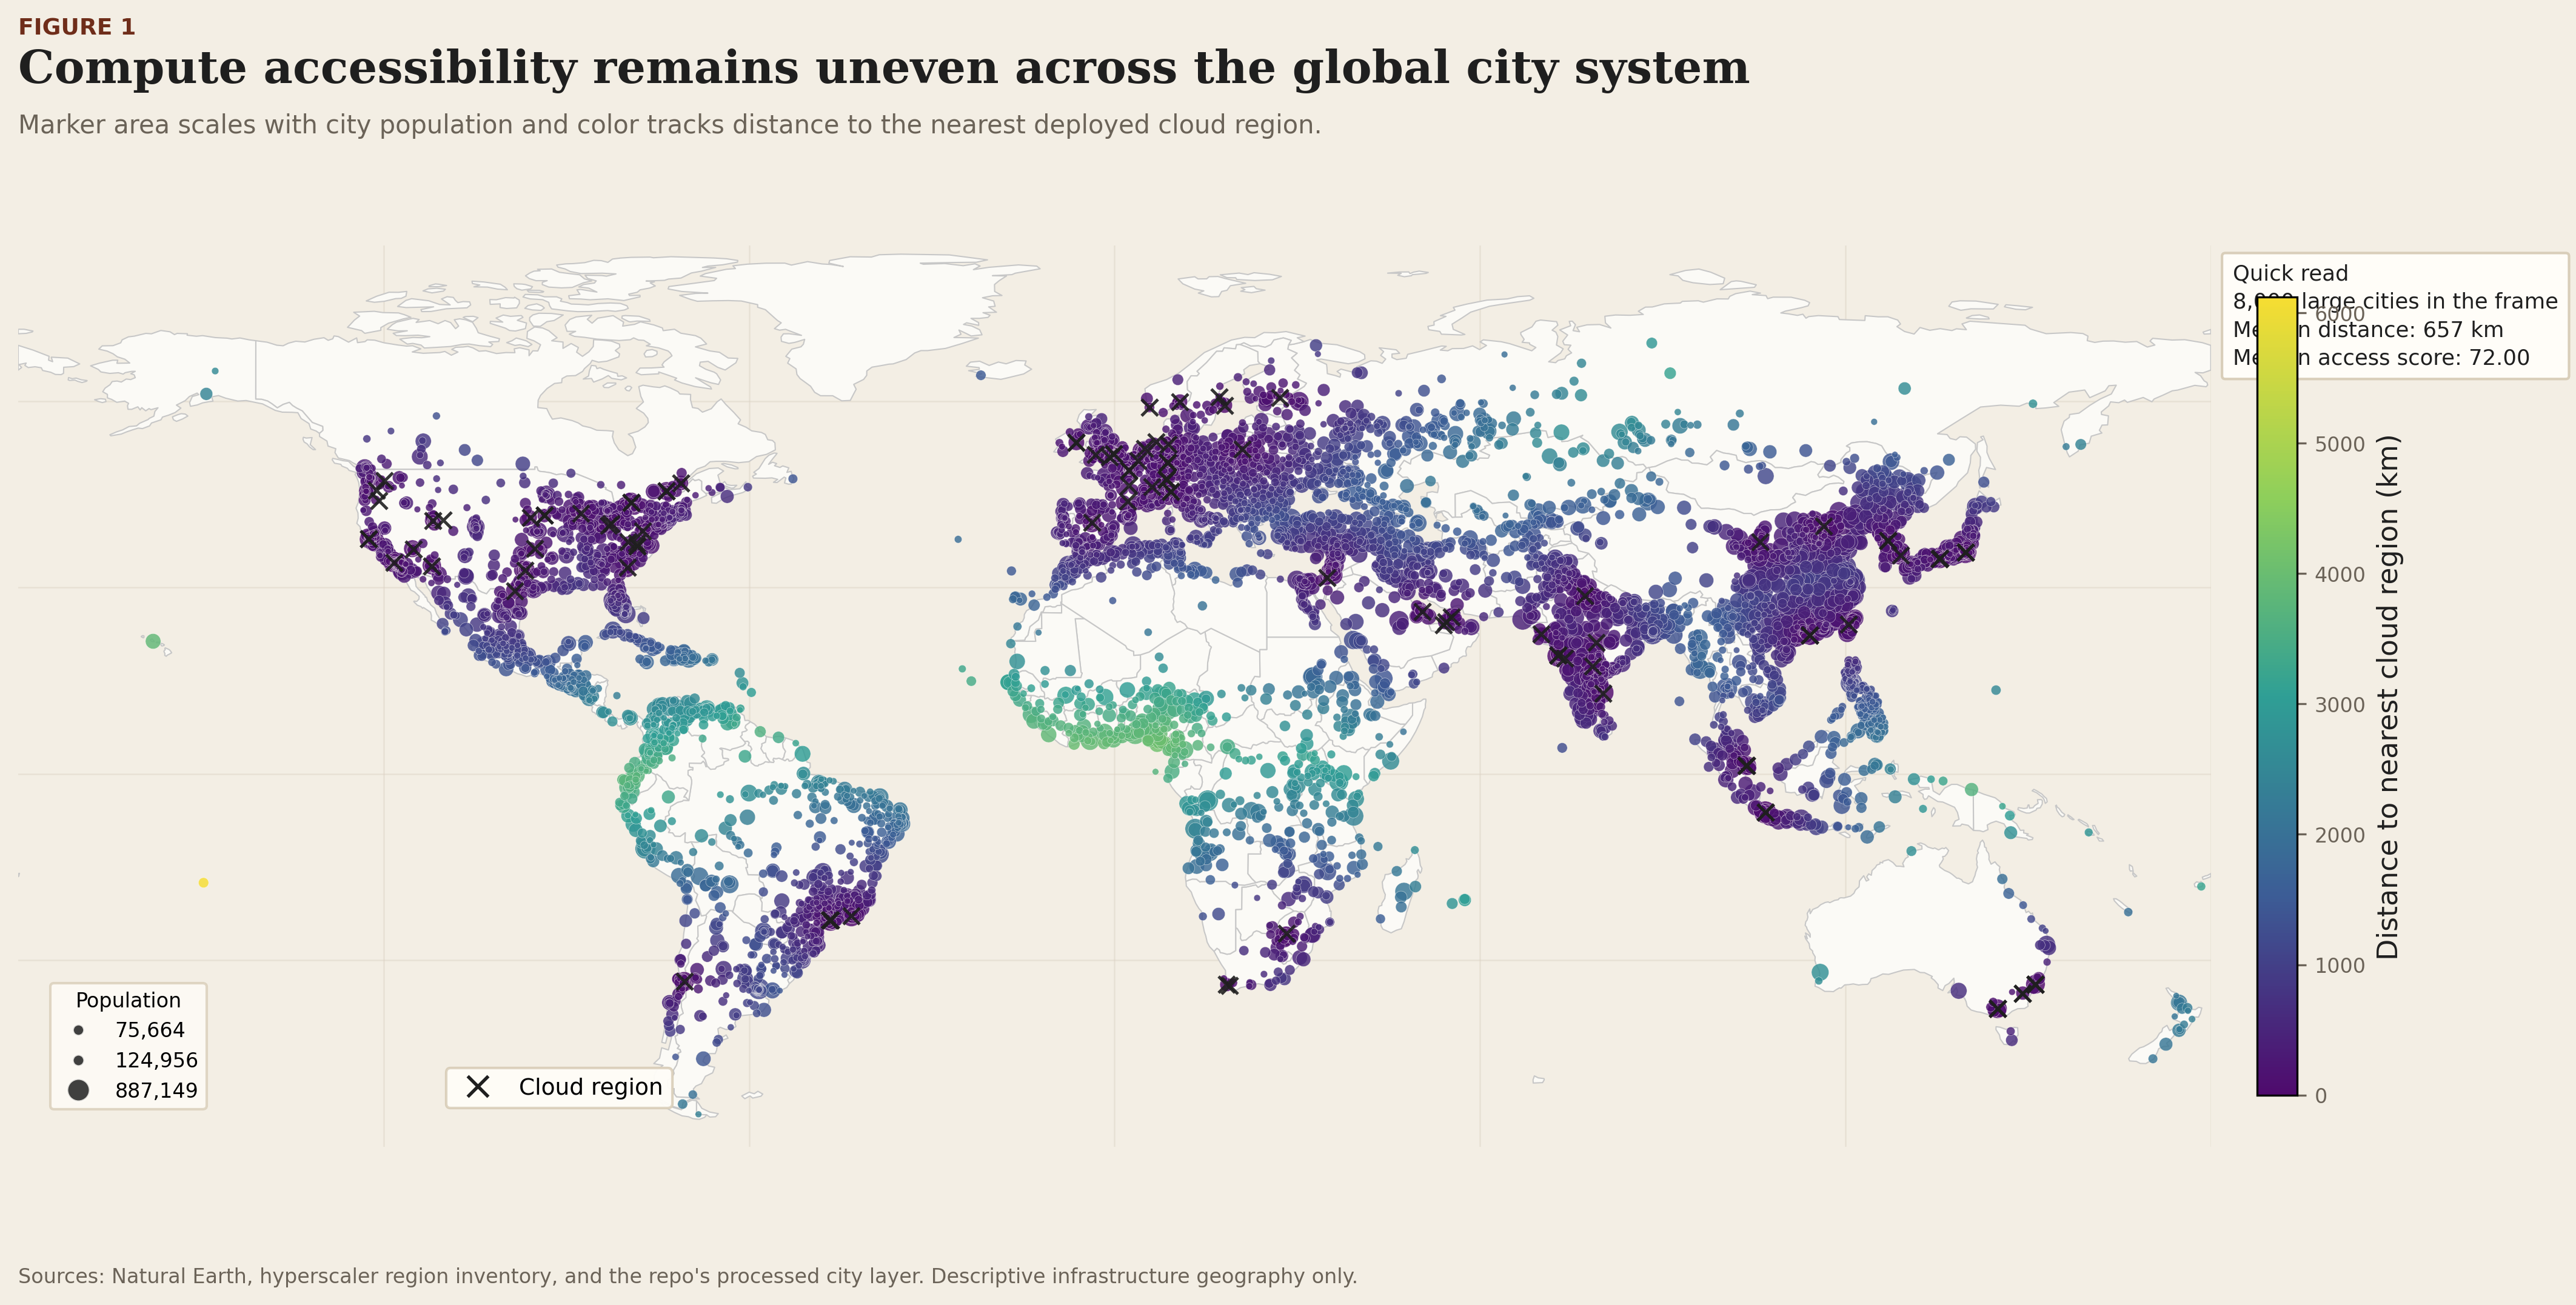
\includegraphics[width=\textwidth]{figures/fig1_access_map.png}
  \caption{Distance from each city in the 8,000-city frame to the nearest AWS, Azure, or Google Cloud region. The map makes the first core point visible: compute access is uneven across the global city system.}
  \label{fig:accessmap}
\end{figure}

That unevenness is not minor. In the rebuilt atlas, the median city in the full 8,000-city frame is about 657 km from its nearest major cloud region. Large parts of the world remain substantially farther away than the dense infrastructure corridors of North America, Europe, and East Asia.

\subsection{The second descriptive fact: AI-linked cities are much closer to compute}
The most readable result in the project appears when the AI-linked subset is compared directly to the full urban frame. Figure~\ref{fig:hist} shows the two distributions.

\begin{figure}[H]
  \centering
  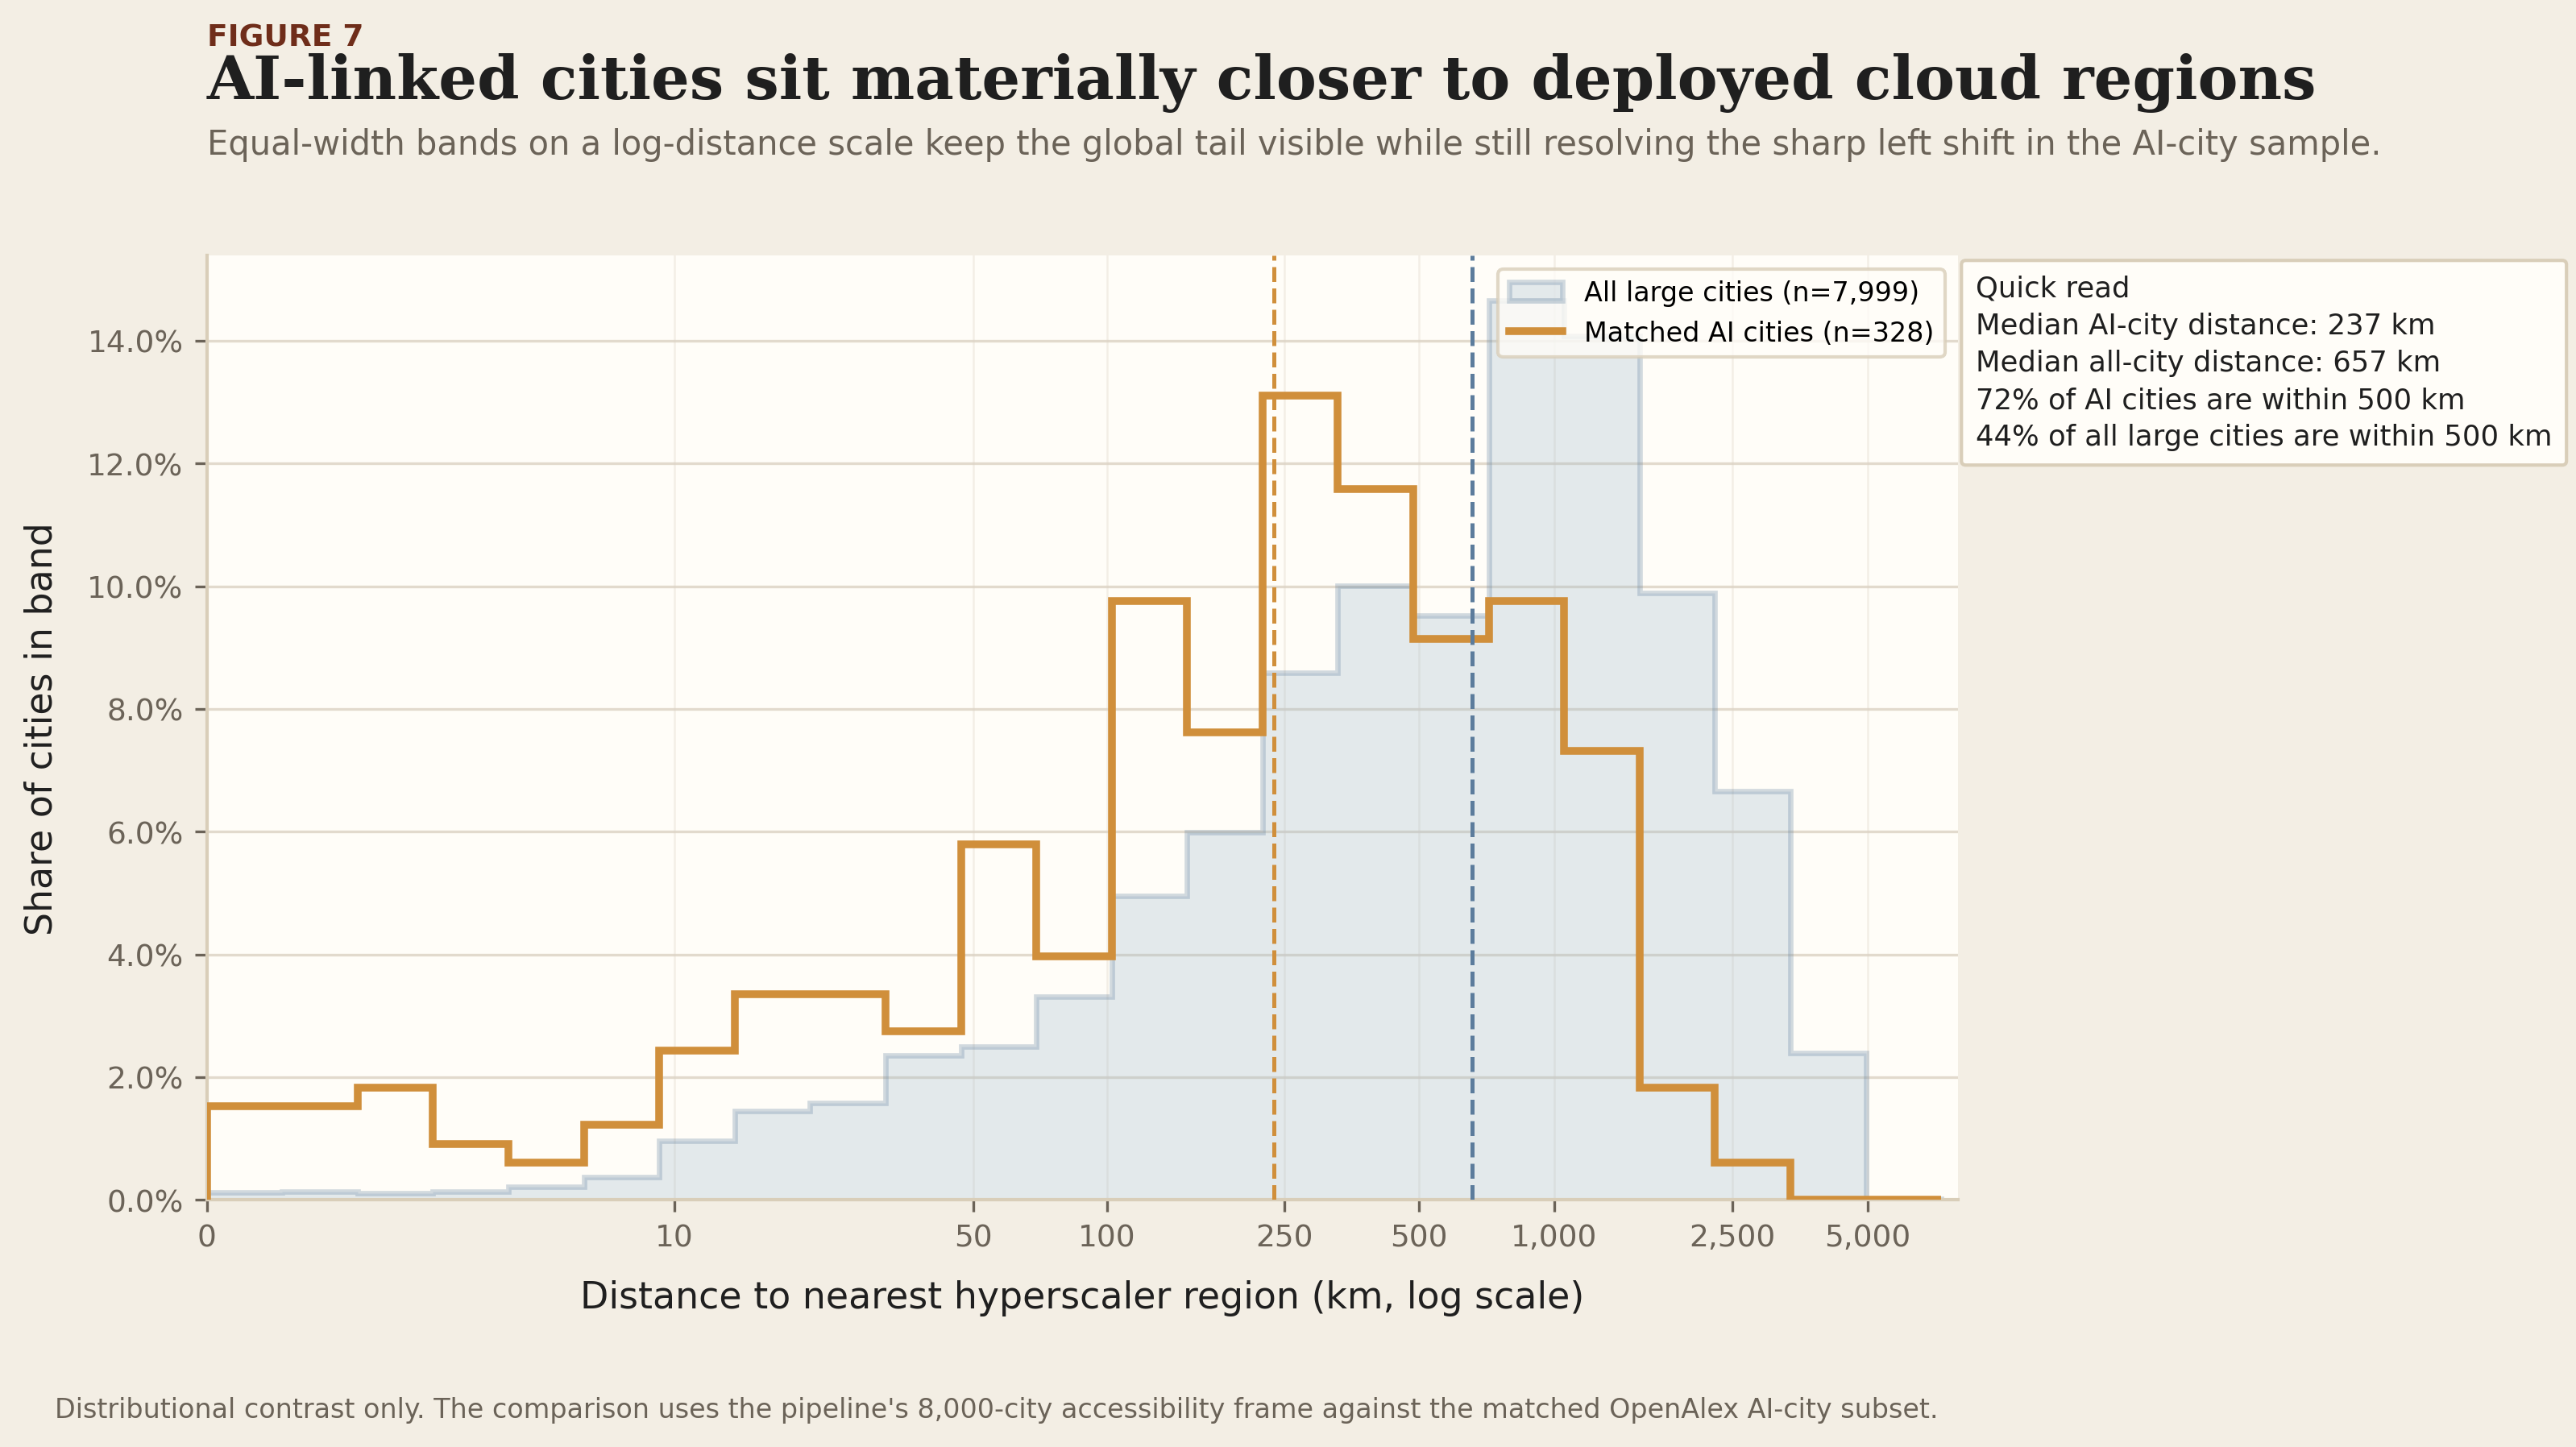
\includegraphics[width=0.92\textwidth]{figures/fig7_distance_hist.png}
  \caption{Distance-to-cloud distributions for the full city frame and the AI-linked city subset. The AI-linked distribution is shifted markedly toward shorter distances.}
  \label{fig:hist}
\end{figure}

The numerical contrast is strong. The median AI-linked city is only about 237 km from its nearest cloud region, compared with about 657 km for the full comparison frame. About 72\% of AI-linked cities fall within 500 km of a cloud region, versus about 44\% of the full city frame. The implication is not subtle: AI-linked cities occupy a different part of the global access landscape.

The pattern strengthens when the overlay is weighted by observed AI works rather than counting each city once.

\begin{figure}[H]
  \centering
  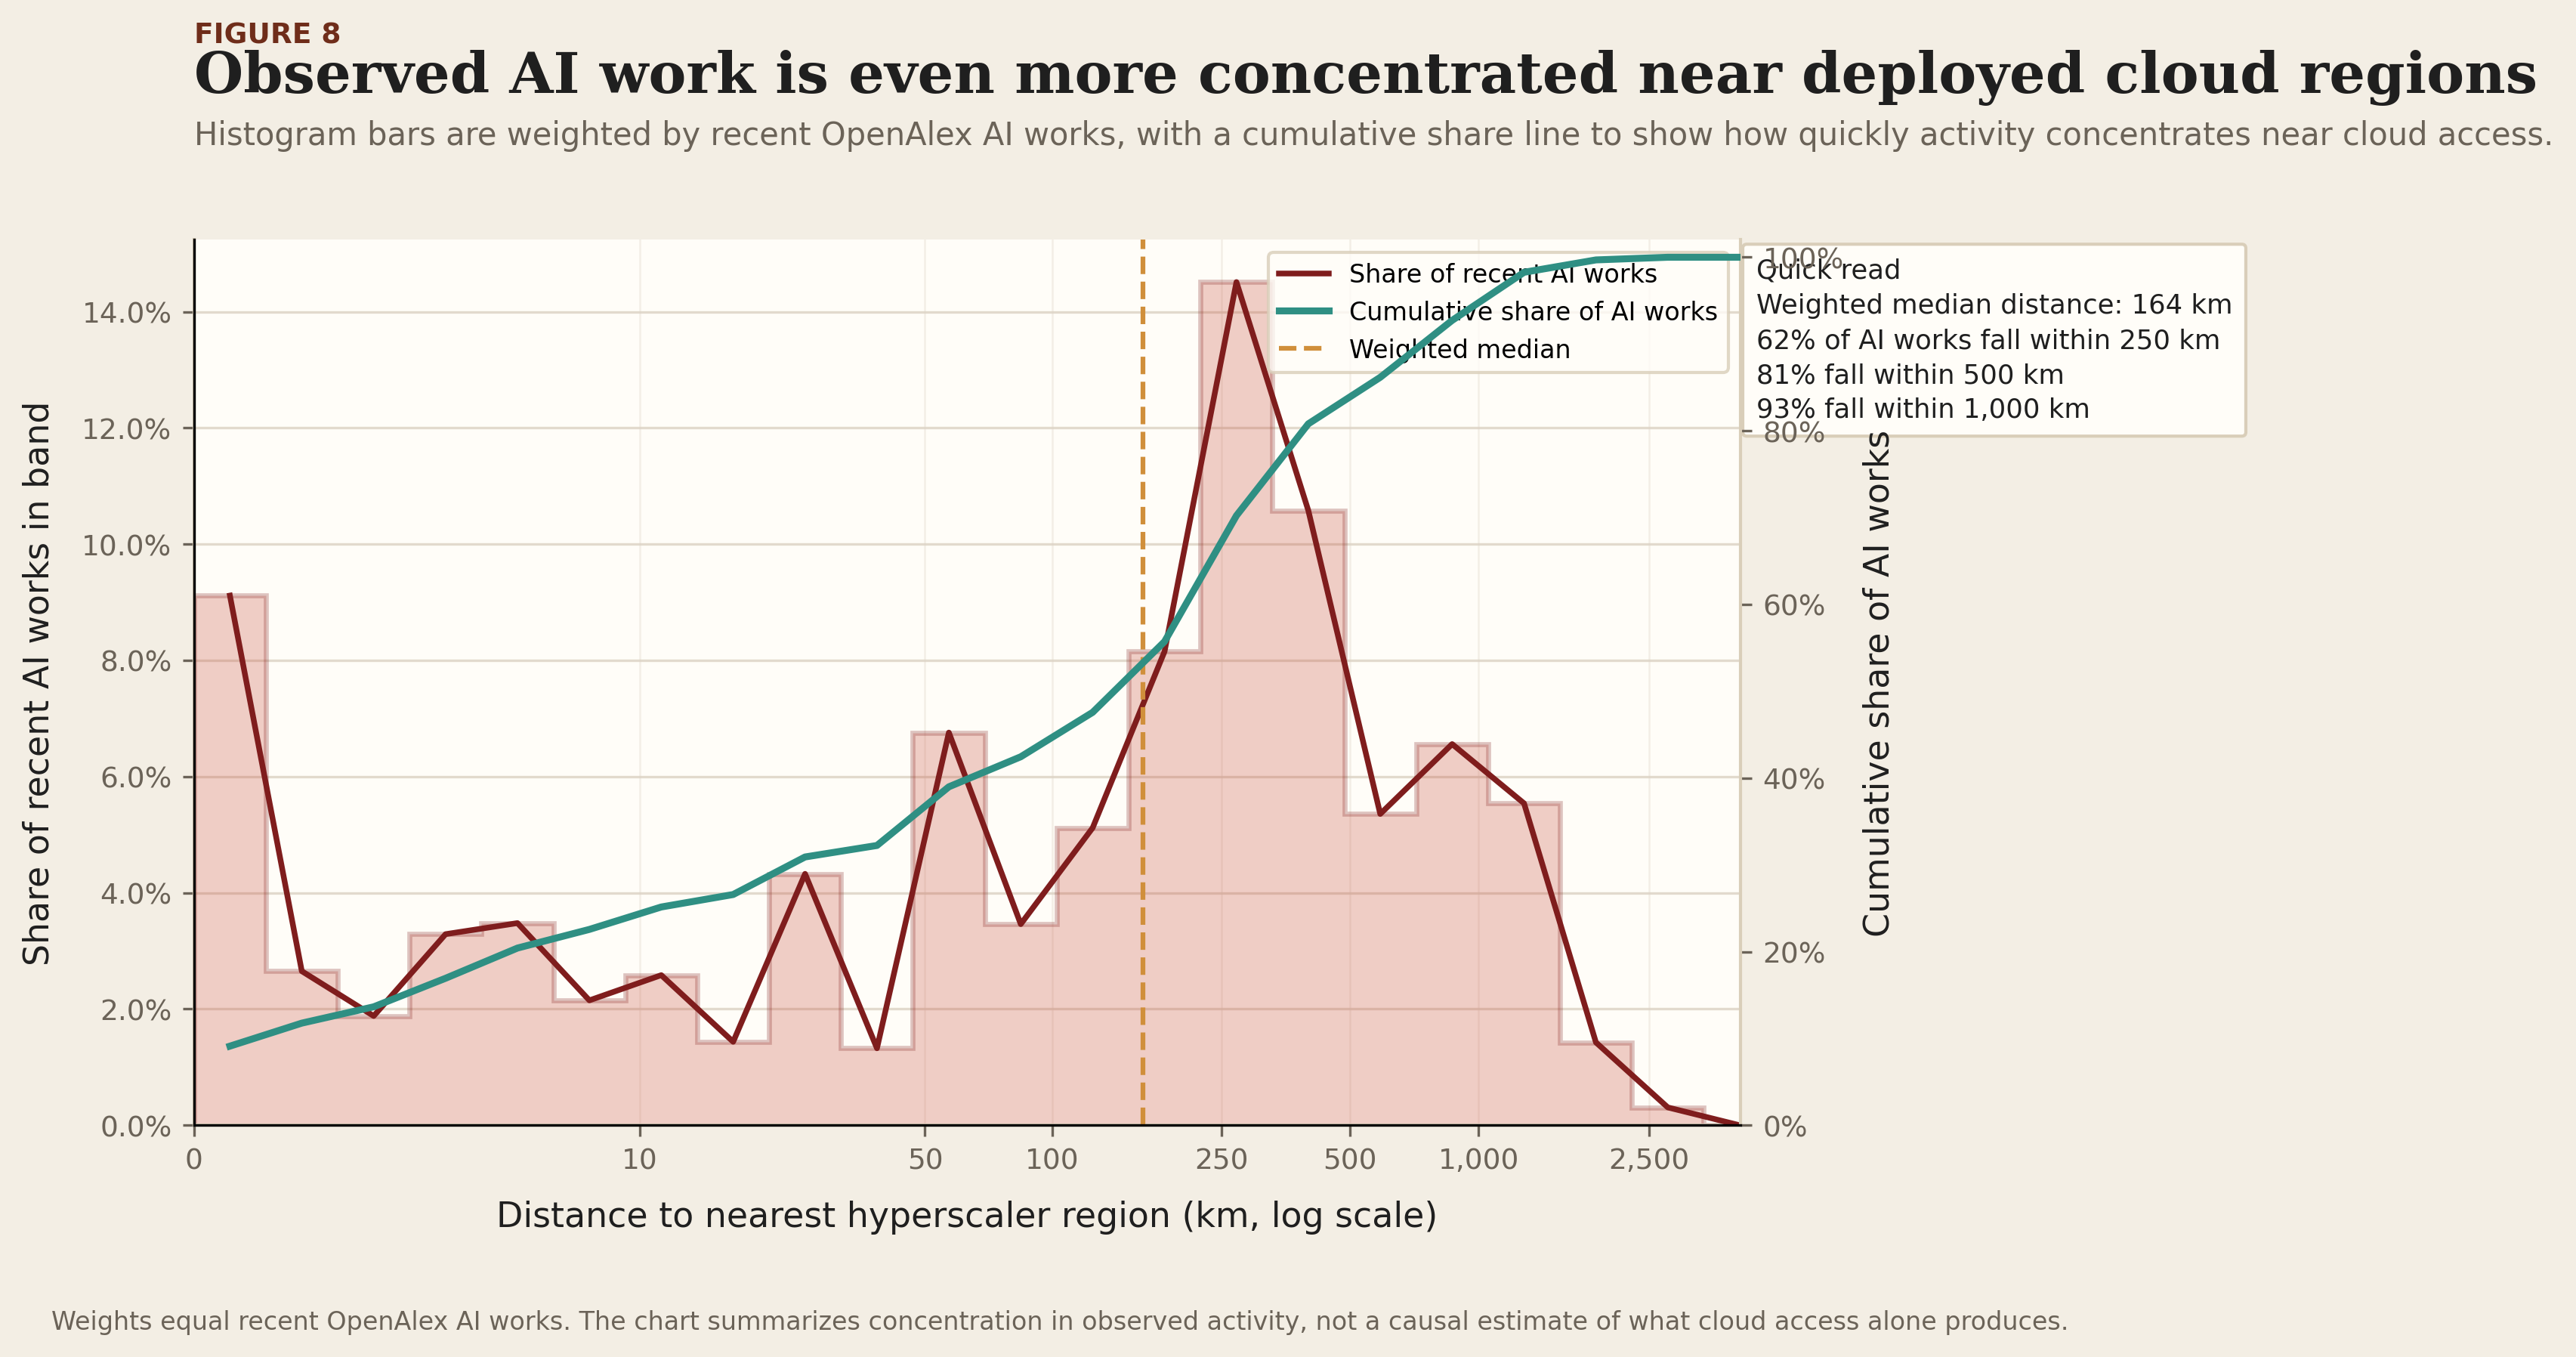
\includegraphics[width=0.92\textwidth]{figures/fig8_ai_weighted_distance.png}
  \caption{Weighted distance profile for observed AI activity. When the overlay is weighted by AI works, the center of gravity moves even closer to cloud infrastructure, with a weighted median of about 164 km.}
  \label{fig:weighted}
\end{figure}

This is an important refinement. The bulk of visible AI research activity is even more compute-proximate than the city-level presence/absence pattern alone suggests.

\subsection{The third descriptive fact: the pattern is spatially organized}
The project does not stop at a histogram. It also checks whether the geography of observed AI activity is spatially clustered. Moran’s $I$ is modest but statistically meaningful: about 0.066 with a permutation $z$-score of about 2.86 and a two-sided $p$-value of 0.008. In plain English, the pattern is not random noise spread across cities.

\begin{figure}[H]
  \centering
  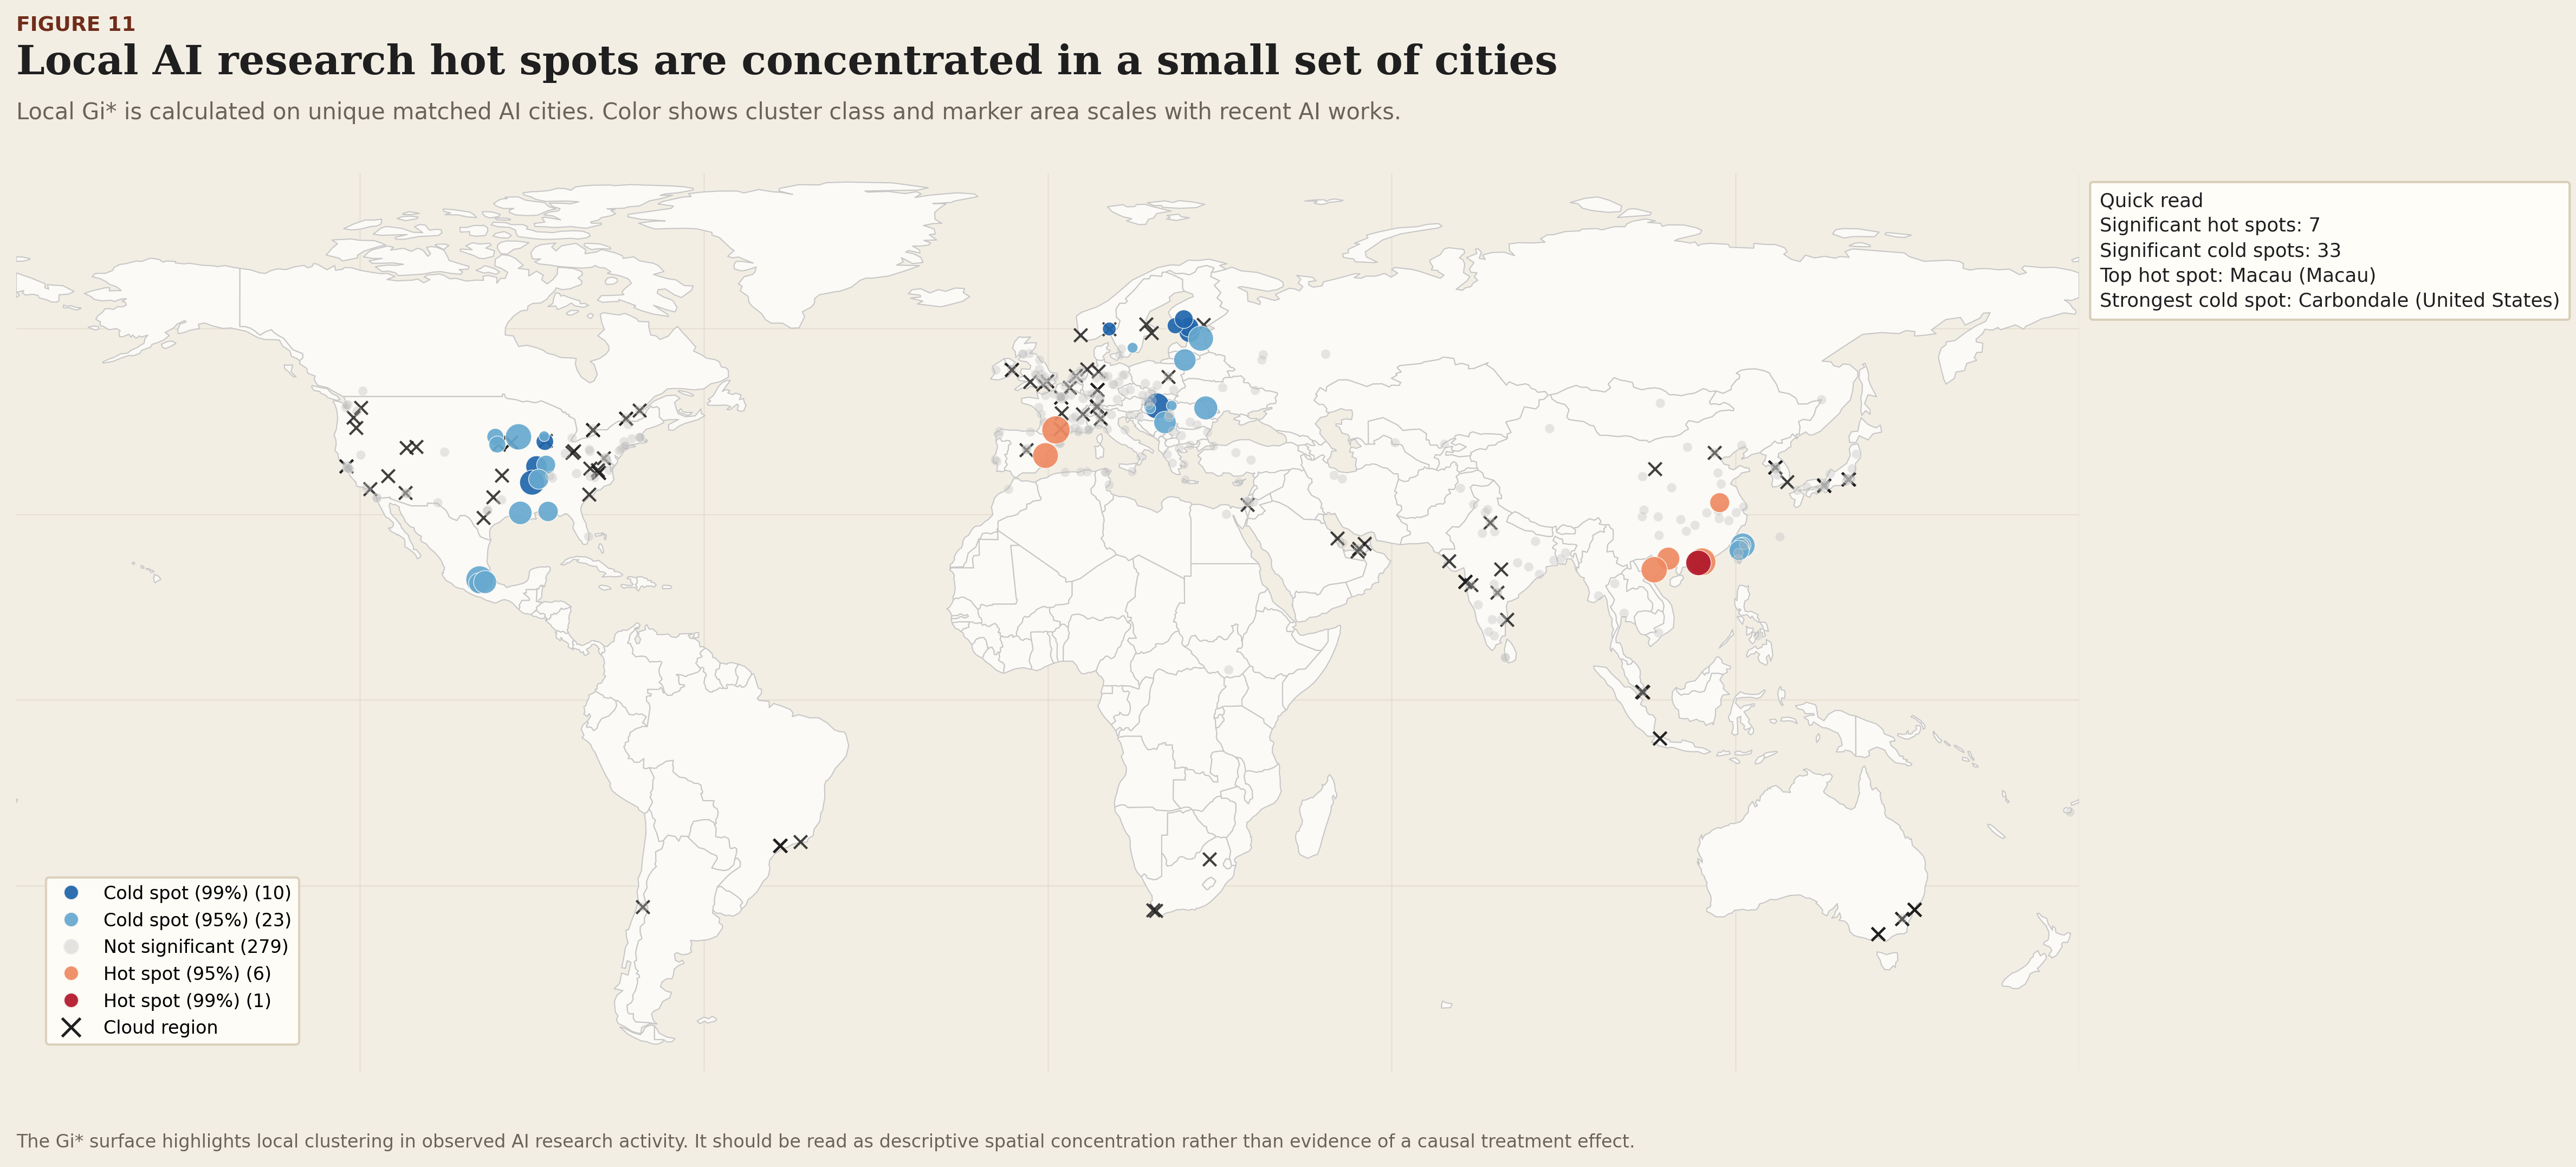
\includegraphics[width=\textwidth]{figures/fig11_hotspot_map.png}
  \caption{Local hot spots and cold spots in the rebuilt atlas. The pattern is geographically structured rather than a collection of isolated famous hubs.}
  \label{fig:hotspots}
\end{figure}

The local hot-spot and cold-spot map makes that structure easier to read. In the rebuilt diagnostics, 7 hot spots and 33 cold spots appear in the unique-city layer used for local Gi$^*$. This is useful because it shows that the compute/AI relationship is spatially organized without claiming that it is spatially uniform.

\subsection{The atlas as a public-interest screening tool}
The final descriptive layer turns the atlas into a practical screening device. The project flags cities with zero observed AI works in the delivered overlay and distance above the current upper-quartile threshold of about 1,251.6 km. That rule yields 1,988 priority cities.

\begin{figure}[H]
  \centering
  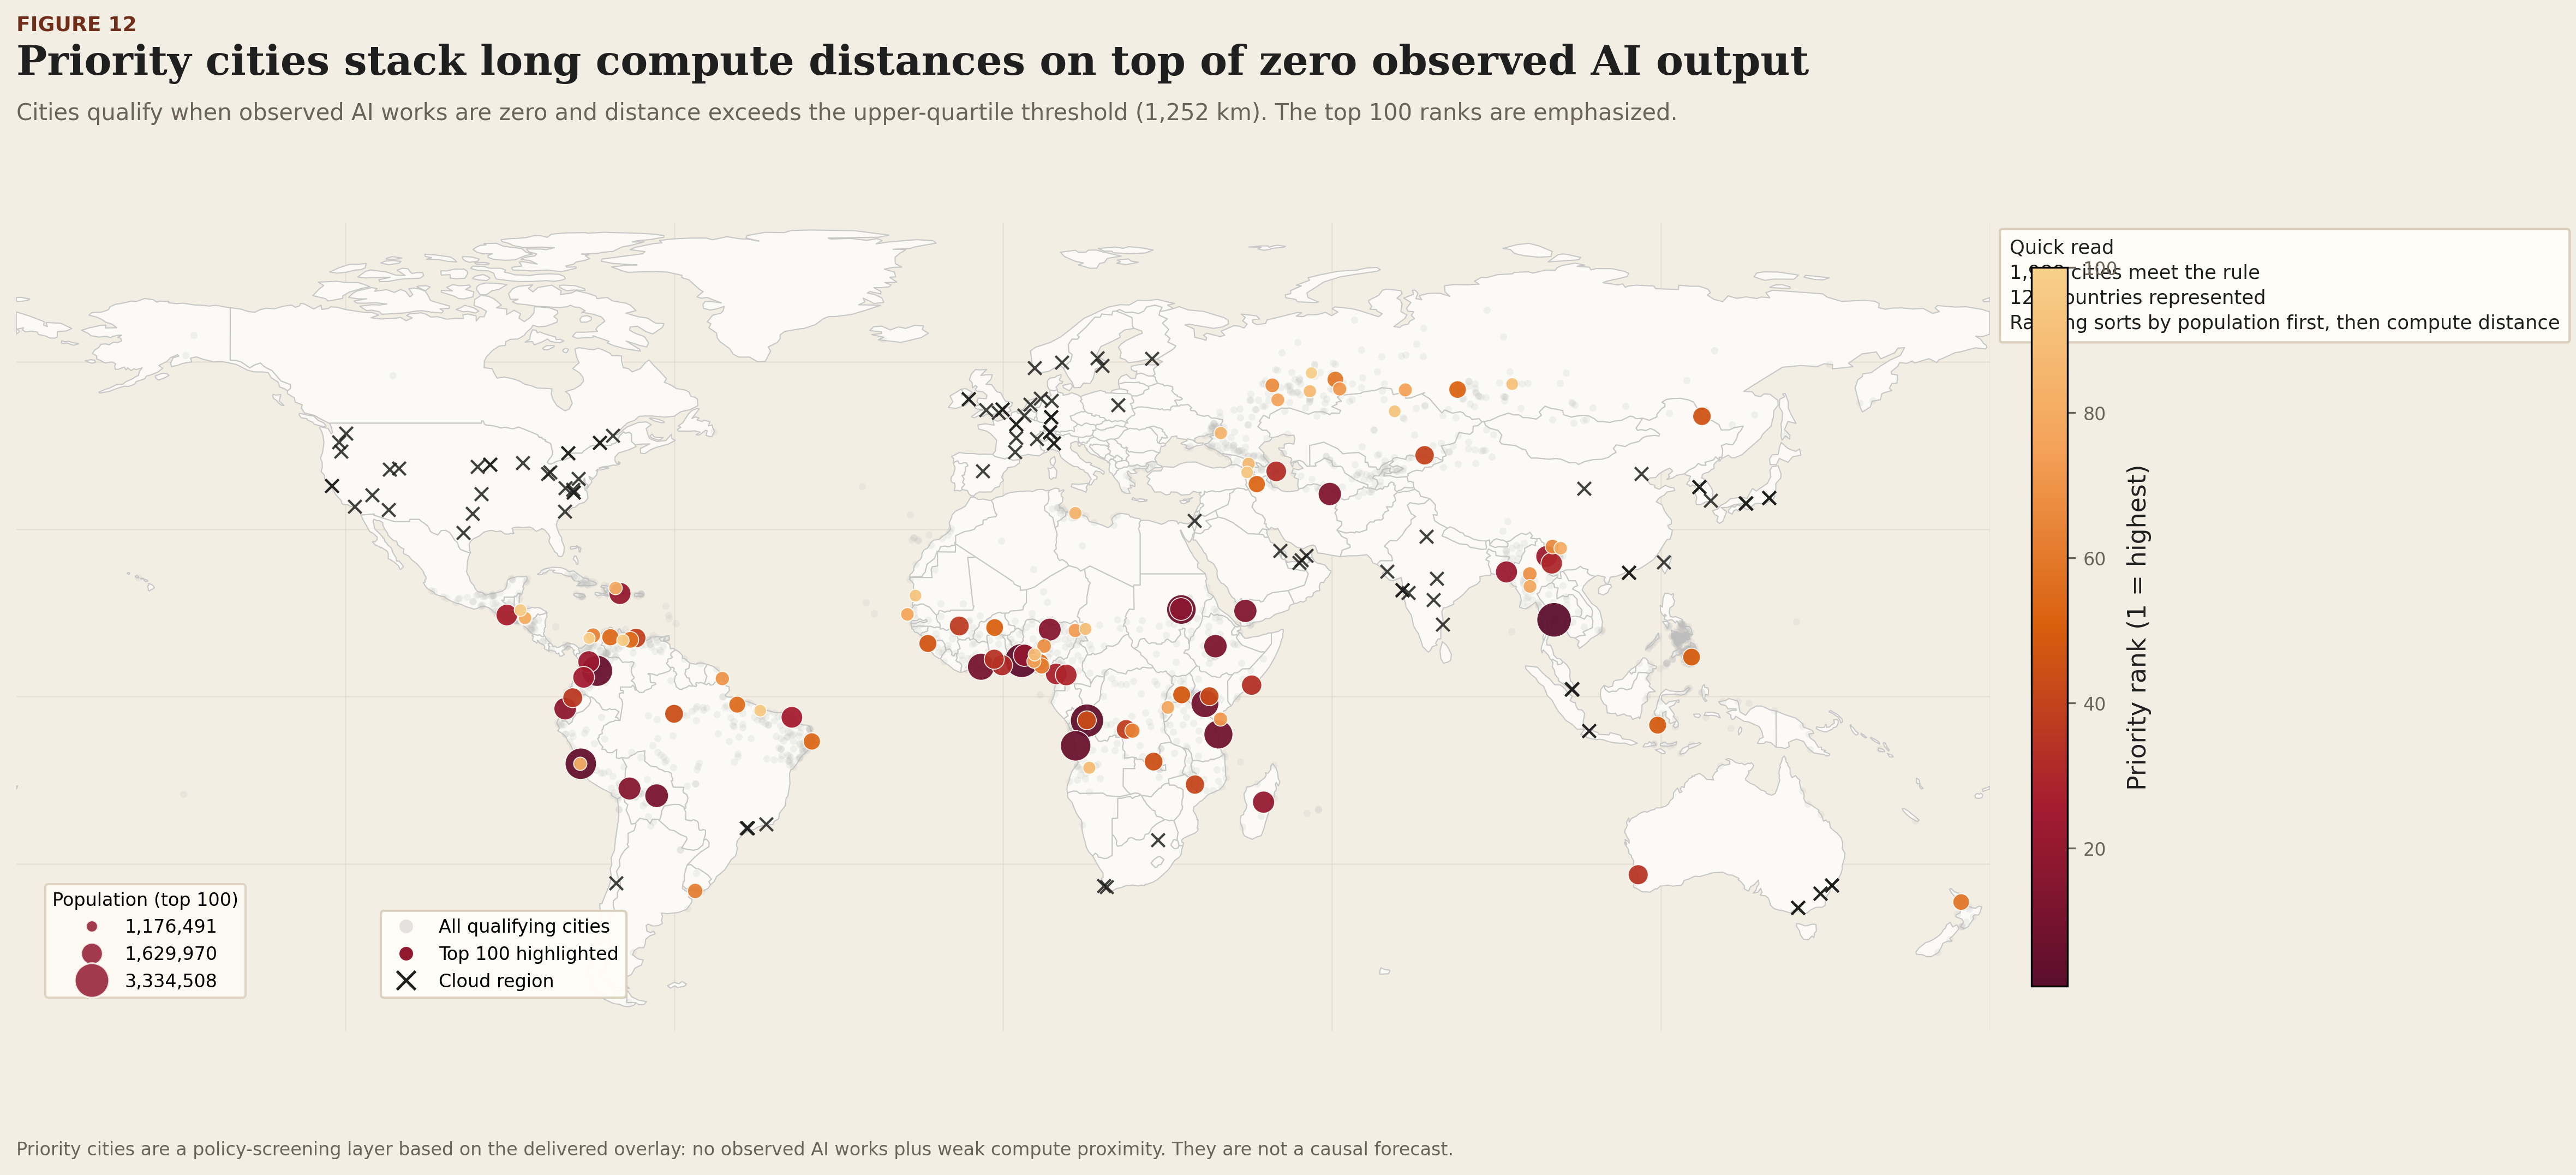
\includegraphics[width=\textwidth]{figures/fig12_priority_cities_map.png}
  \caption{Priority-city screen. Cities are flagged when they combine no observed AI works in the delivered overlay with above-threshold compute distance.}
  \label{fig:priority}
\end{figure}

This layer matters for EIP because it converts the atlas from a descriptive product into a public-interest triage tool. Bangkok, Lagos, Kinshasa, Lima, and Bogot\'a are among the clearest examples in the current build.

\begin{table}[ht]
\centering
\begin{tabular}{llrrll}
\toprule
City & ISO2 & Population (approx) & Dist. to nearest region (km) & Nearest provider & Nearest region \\
\midrule
Bangkok & TH & 17066000 & 1423 & gcp & asia-southeast1 \\
Lagos & NG & 15279000 & 3843 & gcp & europe-southwest1 \\
Kinshasa & CD & 13528000 & 2750 & azure & southafricanorth \\
Lima & PE & 9848000 & 2465 & gcp & southamerica-west1 \\
Bogotá & CO & 9464000 & 3238 & gcp & us-east1 \\
Luanda & AO & 8417000 & 2457 & azure & southafricanorth \\
Khartoum & SD & 7282000 & 1787 & aws & il-central-1 \\
Dar es Salaam & TZ & 6698000 & 2410 & azure & southafricanorth \\
Nairobi & KE & 5545000 & 2870 & azure & southafricanorth \\
Abidjan & CI & 4980000 & 3901 & gcp & europe-southwest1 \\
Santa Cruz & BO & 3151676 & 1821 & gcp & southamerica-east1 \\
Addis Ababa & ET & 3041002 & 2275 & aws & me-south-1 \\
\bottomrule
\end{tabular}
\caption{Illustrative 'AI deserts': large cities with zero AI works under the selected OpenAlex topic filter, and far from hyperscaler regions (distance $\geq$ 75th percentile).}
\label{tab:underserved}
\end{table}


\section{Spatial diagnostics and model checks: what remains after basic controls}
The project uses two spatial model specifications to check whether the negative distance pattern survives basic controls for population and geography. The first is a driver regression with a Gaussian Process residual surface, which absorbs broad smooth regional structure \citep{rasmussen2006}. The second is a driver regression with a CAR/GMRF-style neighborhood term, which absorbs stronger local dependence across an eight-nearest-neighbor graph \citep{besag1974,rue2005}.

\begin{table}[ht]
\centering
\begin{tabular}{lll}
\toprule
Term & GP+drivers ($\beta$) & CAR/GMRF+drivers ($\beta$) \\
\midrule
Distance to nearest region (per 1000 km) & -0.207 & -0.052 \\
City size (log population) & +0.279 & +0.309 \\
\bottomrule
\end{tabular}
\caption{Model coefficient comparison (posterior mean / empirical Bayes). Outcome is log(1 + AI works).}
\label{tab:model_coefs}
\end{table}


\begin{figure}[H]
  \centering
  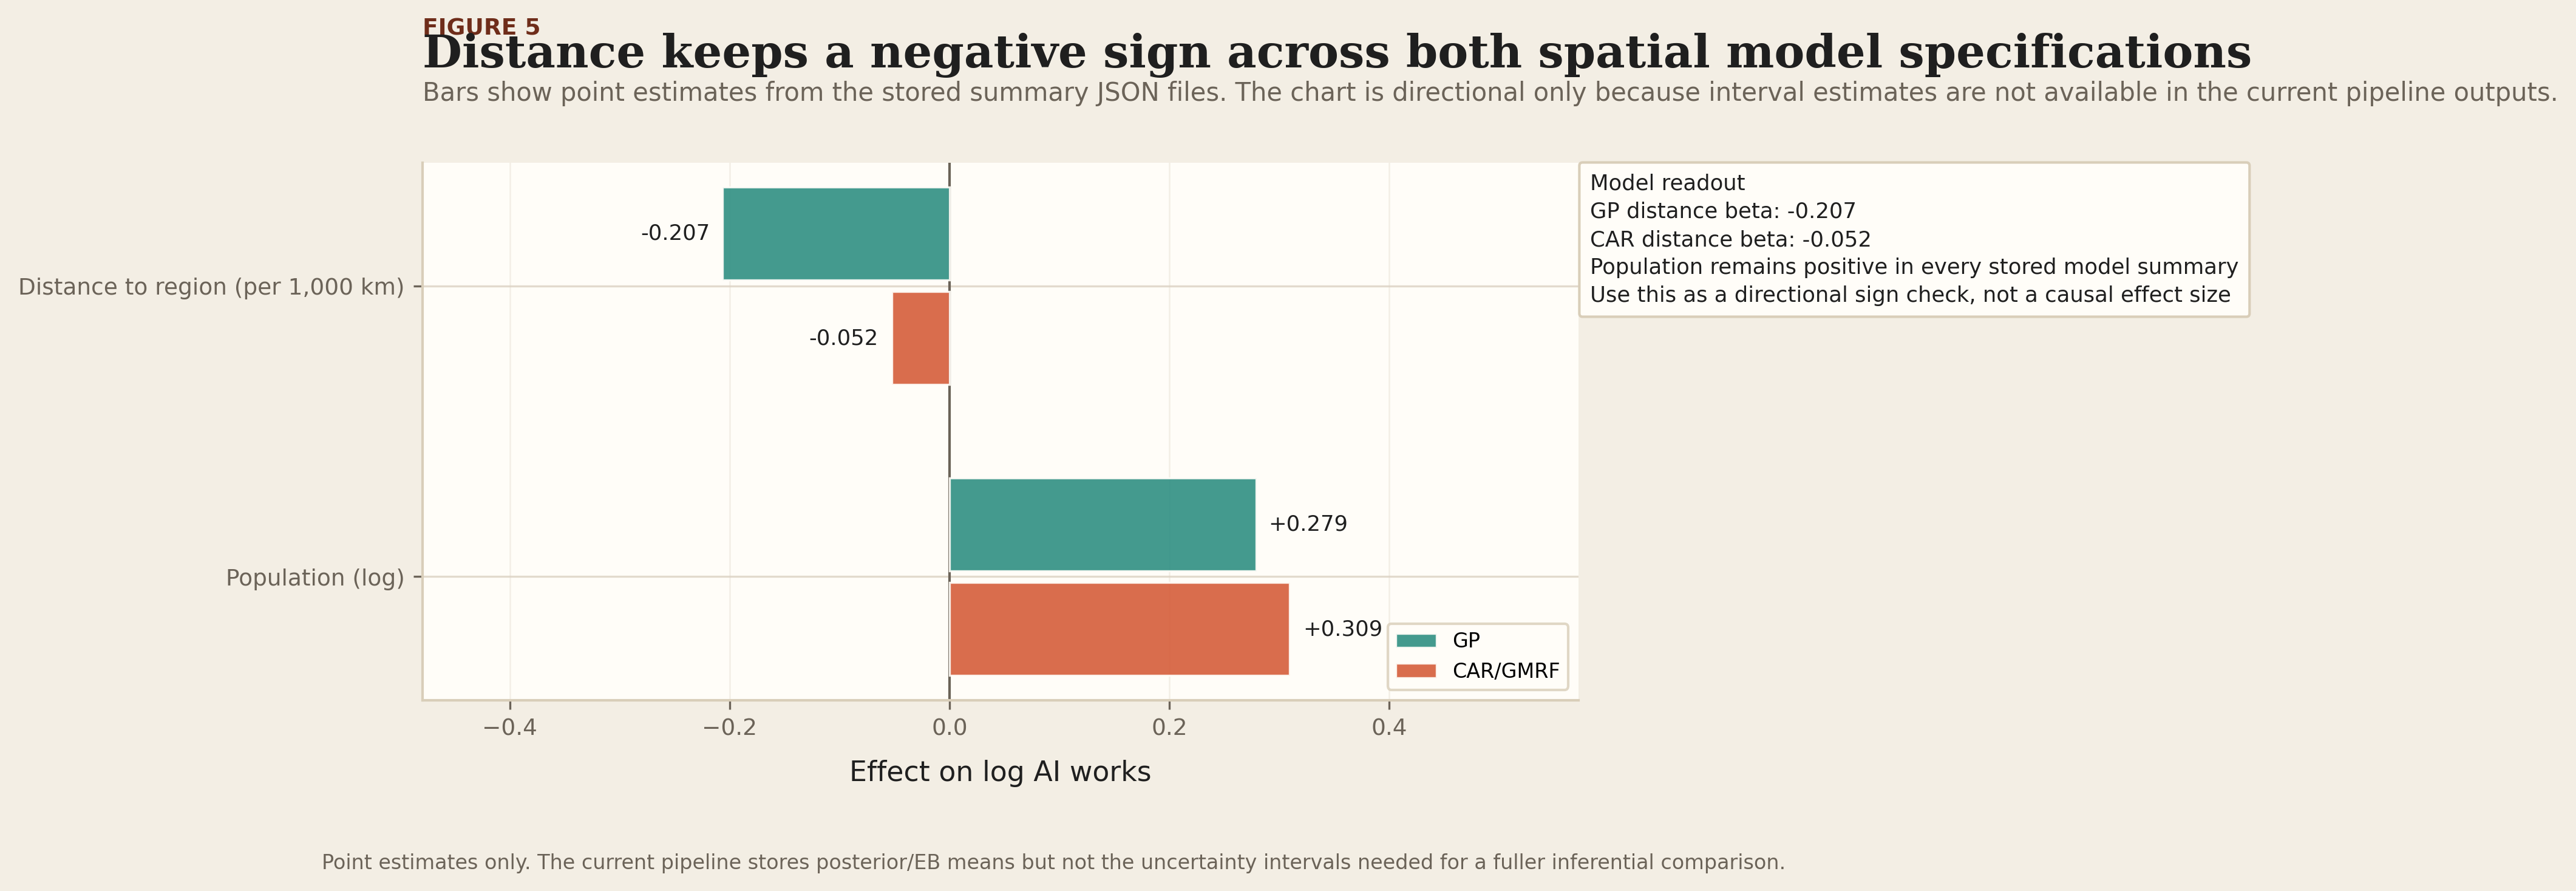
\includegraphics[width=0.9\textwidth]{figures/fig5_coef_compare.png}
  \caption{Distance and population coefficients in the two spatial models. The distance coefficient stays negative and the population coefficient stays positive in both specifications.}
  \label{fig:coefcompare}
\end{figure}

The exact coefficients differ, which is informative rather than contradictory. In the GP model, the distance coefficient is about $-0.207$ per additional 1,000 km. In the CAR/GMRF model, it shrinks to about $-0.052$. The sign remains negative, but the magnitude attenuates once stronger local spatial structure is absorbed. That is the right interpretation for this submission: part of the raw distance gradient overlaps with broader regional ecosystems, yet the relationship does not vanish.

The point is not to crown one model as the final truth. The point is to show that the descriptive finding survives two materially different ways of handling geography. That strengthens the project’s credibility while still leaving room for honest caution.

\section{Beyond distance: the Compute Opportunity Bundle Index}
\subsection{Why the final submission needed an originality layer}
The existing atlas already had a strong descriptive backbone. What it lacked was a visibly original analytical layer that could deepen the project without dragging it away from readability. Two candidate originality packages were prototyped for the final pass: a counterfactual siting layer and a composite bundle layer. The bundle layer won because it had the best combination of novelty, StoryMap legibility, and fit with the project’s actual claim.

The resulting Compute Opportunity Bundle Index is the main originality contribution of the final submission. It answers a sharper question than raw distance alone: which cities are merely close to one cloud region, and which cities sit inside a broader compute-opportunity environment built from proximity, provider diversity, regional redundancy, institutional anchors, and city scale?

\begin{table}[ht]
\centering
\small
\begin{tabular}{p{0.33\textwidth}cp{0.43\textwidth}}
\toprule
Component & Weight & Interpretation \\ 
\midrule
Nearest-region proximity & 0.40 & Closer cities receive higher standardized access scores \\ 
Provider diversity within 1,000 km & 0.15 & Cities near more providers receive higher scores \\ 
Regional redundancy within 1,500 km & 0.15 & Cities near more total regions receive higher scores \\ 
City scale (population) & 0.15 & Larger cities receive a modest scale boost \\ 
Institutional anchors & 0.15 & Cities with stronger OpenAlex-linked AI institutions score higher \\ 
\bottomrule
\end{tabular}
\caption{Compute Opportunity Bundle Index components and weights. All components are standardized to a 0--1 range before weighting, then combined into a 0--100 bundle score.}
\label{tab:bundle_weights}
\end{table}


\subsection{How the bundle index is constructed}
The index is intentionally conservative. It uses only layers already validated in the project workspace:
\begin{itemize}[leftmargin=*]
  \item nearest-region cloud proximity,
  \item provider diversity within 1,000 km,
  \item total regional redundancy within 1,500 km,
  \item institutional anchor strength from the delivered OpenAlex-linked files,
  \item and city scale as a modest weighting component.
\end{itemize}

Each component is standardized to a common range before weighting. The result is a 0--100 score that does not replace the atlas backbone; it sharpens it.

\begin{figure}[H]
  \centering
  
\includegraphics[width=\textwidth]{../final_submission/originality/final/fig_bundle_index_map.png}
  \caption{Compute Opportunity Bundle Index. The index extends the project beyond raw nearest-region distance by incorporating provider diversity, regional redundancy, institutional anchoring, and city scale.}
  \label{fig:bundlemap}
\end{figure}

\subsection{What the bundle layer adds}
The bundle layer contributes three things. First, it creates a second global map that is still easy to read but conceptually richer than distance alone. Second, it creates a comparison view between a distance-only score and the broader bundle score. Third, it creates a ranking layer that helps distinguish cities that are merely compute-proximate from cities that sit inside deeper opportunity structures.

\begin{figure}[H]
  \centering
  
\includegraphics[width=0.82\textwidth]{../final_submission/originality/final/fig_bundle_vs_distance.png}
  \caption{Distance-only access versus bundle score. The bundle index does not discard proximity; it shows which cities rise or fall once redundancy and institutional anchoring are added.}
  \label{fig:bundlevsdist}
\end{figure}

\begin{figure}[H]
  \centering
  
\includegraphics[width=0.82\textwidth]{../final_submission/originality/final/fig_bundle_top_cities.png}
  \caption{Top cities by bundle score. The highest-ranked cities are not simply the cities nearest to one cloud region; they are cities where proximity, redundancy, and institutional depth reinforce one another.}
  \label{fig:bundletop}
\end{figure}

In the rebuilt final outputs, the highest-scoring bundle cities include Paris, Tokyo, London, Beijing, Barcelona, New York, Toronto, Amsterdam, Warsaw, and Berlin. That list is revealing. It is not identical to the pure nearest-distance ranking. The bundle layer rewards places where multiple providers, more regional redundancy, and stronger institutional anchoring accumulate in the same urban system.

This is the most important originality result in the submission. It gives the report a more ambitious but still honest claim: not only is compute access uneven, but some cities occupy broader bundles of compute opportunity than others, even among cities that look similarly close to one region on a raw distance map.

\section{Four cities that explain the pattern}
The atlas-wide results matter, but they are not enough on their own. A strong EIP story also needs place-based explanation. The four final cases therefore translate the quantitative backbone into readable urban logic. Each case uses two map plates: a regional context map and a local ecosystem map. Together, they show why distance matters, why it is not everything, and why the bundle framing is more useful than a single-variable story.

\begin{table}[ht]
\centering
\small
\begin{tabular}{p{0.18\textwidth}p{0.18\textwidth}rrrp{0.23\textwidth}}
\toprule
City & Quadrant & Distance (km) & Bundle score & AI works & Key takeaway \\ 
\midrule
Singapore & near compute / high AI & 4.1 & 85.7 & 1072 & Alignment benchmark \\ 
Seoul & near compute / low AI & 1.3 & 84.0 & 10 & Overlay-limit exception \\ 
Ho Chi Minh City & far compute / high AI & 1096.8 & 61.7 & 373 & Outperforms distance-only expectation \\ 
Lagos & far compute / low AI & 3842.6 & 27.8 & 0 & Stacked-disadvantage priority city \\ 
\bottomrule
\end{tabular}
\caption{Final four-city case matrix used in the report and StoryMap.}
\label{tab:case_matrix}
\end{table}


\subsection{Singapore: near compute, high AI}
Singapore is the alignment benchmark in the final report. It sits only about 4.1 km from the nearest major cloud region, has three providers within 1,000 km, five regions within 1,500 km, four top-institution anchors, and 1,072 recent AI works attached to those anchors in the delivered files. Its bundle score is 85.7.

\begin{figure}[H]
  \centering
  \begin{subfigure}[t]{0.48\textwidth}
    \centering
    
\includegraphics[width=\textwidth]{../final_submission/case_studies/singapore/regional_context/singapore_regional_context.png}
    \caption{Regional context.}
  \end{subfigure}\hfill
  \begin{subfigure}[t]{0.48\textwidth}
    \centering
    
\includegraphics[width=\textwidth]{../final_submission/case_studies/singapore/local_ecosystem/singapore_local_ecosystem.png}
    \caption{Local ecosystem.}
  \end{subfigure}
  \caption{Singapore case-study plates. Singapore shows what a fully reinforced compute-opportunity bundle looks like in the project’s current data.}
  \label{fig:singaporecase}
\end{figure}

Singapore matters because it shows the project’s main pattern in its strongest form. Compute access is extremely strong, redundancy is high, institutional anchoring is strong, and the city’s visible AI activity is correspondingly high. This is not proof that compute caused Singapore’s position. It is evidence that the bundle logic is coherent.

\subsection{Seoul: near compute, low AI in the delivered overlay}
Seoul is the key exception case. It sits only about 1.3 km from the nearest cloud region and has three providers within 1,000 km and 11 regions within 1,500 km, yet it has only 10 recent AI works and one top-institution anchor in the delivered overlay. Its bundle score is still very high at 84.0.

\begin{figure}[H]
  \centering
  \begin{subfigure}[t]{0.48\textwidth}
    \centering
    
\includegraphics[width=\textwidth]{../final_submission/case_studies/seoul/regional_context/seoul_regional_context.png}
    \caption{Regional context.}
  \end{subfigure}\hfill
  \begin{subfigure}[t]{0.48\textwidth}
    \centering
    
\includegraphics[width=\textwidth]{../final_submission/case_studies/seoul/local_ecosystem/seoul_local_ecosystem.png}
    \caption{Local ecosystem.}
  \end{subfigure}
  \caption{Seoul case-study plates. Seoul is the strongest reminder that the delivered research overlay is not the whole AI economy.}
  \label{fig:seoulcase}
\end{figure}

Seoul earns its place because it keeps the submission honest. A compute-rich city can still look comparatively quiet in the delivered overlay. That does not weaken the atlas. It clarifies what the atlas is measuring. Seoul is therefore the project’s strongest overlay-limit case.

\subsection{Ho Chi Minh City: far compute, high AI}
Ho Chi Minh City is the clearest city that beats the raw distance pattern. It sits about 1,096.8 km from the nearest cloud region and has no providers within 1,000 km, yet it shows 373 recent AI works and two top-institution anchors. Its bundle score is 61.7 --- well below the strongest compute hubs, but materially above a city like Lagos.

\begin{figure}[H]
  \centering
  \begin{subfigure}[t]{0.48\textwidth}
    \centering
    
\includegraphics[width=\textwidth]{../final_submission/case_studies/ho_chi_minh_city/regional_context/ho_chi_minh_city_regional_context.png}
    \caption{Regional context.}
  \end{subfigure}\hfill
  \begin{subfigure}[t]{0.48\textwidth}
    \centering
    
\includegraphics[width=\textwidth]{../final_submission/case_studies/ho_chi_minh_city/local_ecosystem/ho_chi_minh_city_local_ecosystem.png}
    \caption{Local ecosystem.}
  \end{subfigure}
  \caption{Ho Chi Minh City case-study plates. This is the project’s strongest ``beats-the-pattern'' case.}
  \label{fig:hcmccase}
\end{figure}

This case is crucial because it prevents the report from sounding deterministic. Distance matters, but it does not settle the story. Ho Chi Minh City shows that institutional anchoring and city-level momentum can offset weaker proximity.

\subsection{Lagos: far compute, low AI}
Lagos is the project’s stacked-disadvantage case. It is one of the largest urban centers in the atlas, yet it sits about 3,842.6 km from the nearest cloud region, has no providers within 1,000 km, no regions within 1,500 km, no top-institution anchors in the delivered files, and zero observed AI works in the overlay. Its bundle score is only 27.8.

\begin{figure}[H]
  \centering
  \begin{subfigure}[t]{0.48\textwidth}
    \centering
    
\includegraphics[width=\textwidth]{../final_submission/case_studies/lagos/regional_context/lagos_regional_context.png}
    \caption{Regional context.}
  \end{subfigure}\hfill
  \begin{subfigure}[t]{0.48\textwidth}
    \centering
    
\includegraphics[width=\textwidth]{../final_submission/case_studies/lagos/local_ecosystem/lagos_local_ecosystem.png}
    \caption{Local ecosystem.}
  \end{subfigure}
  \caption{Lagos case-study plates. Lagos turns the atlas into a public-interest urban-infrastructure story rather than a purely academic one.}
  \label{fig:lagoscase}
\end{figure}

Lagos matters because it makes the stakes visible. It is not a small or marginal city. It is a major urban system that the atlas flags as far from compute and weak in the delivered overlay. This is exactly the kind of case that makes the priority-city screen useful.

\subsection{What the four cases show together}
Together, the four cases do the explanatory work that the regression alone cannot do. Singapore shows alignment. Seoul shows that the delivered overlay is not the whole AI economy. Ho Chi Minh City shows that cities can outperform what distance alone would predict. Lagos shows how weak compute proximity and weak institutional anchoring can stack together in a large city. That is why the report’s final claim is about bundles rather than single causes.

\section{Why this matters for EIP}
A strong EIP submission needs more than coefficients. It needs a visible public-interest problem, a geospatial method that is easy to understand, a polished output, and a conclusion that is both useful and honest. This project’s value for EIP is that it turns an abstract digital-infrastructure problem into a concrete urban geography.

Three practical uses stand out:
\begin{enumerate}[leftmargin=*]
  \item \textbf{Screening.} The atlas shows where large cities appear to face the greatest mismatch between urban scale, compute proximity, and observed AI activity.
  \item \textbf{Explanation.} The bundle index and the four cases explain why distance matters without pretending that it is destiny.
  \item \textbf{Communication.} The project provides a map-first way to discuss AI opportunity that is understandable to non-specialists and still rigorous enough to withstand technical scrutiny.
\end{enumerate}

In that sense, the final report is not simply a technical supplement to a StoryMap. It is the long-form judged artifact that explains why the maps matter.

\section{What the project does not claim}
This section is as important as the results themselves. The submission does not claim that cloud proximity alone determines whether a city succeeds in AI. It does not claim that every city far from compute is excluded, or that every city near compute will become an AI hub. It does not claim that the delivered overlay captures the whole AI economy. And it does not present a definitive causal estimate of cloud-region placement.

The causal extensions were re-audited during the final submission pass. They remain mixed, specification-sensitive, and not strong enough to support a headline treatment-effect claim. The right use of that work is therefore to set a careful evidentiary boundary: the atlas is stronger than a map-level coincidence and weaker than a causal proof. That boundary makes the main claim more believable, not less.

\section{Limitations and future directions}
The project’s limits should be read as next questions, not as hidden defects.
\begin{itemize}[leftmargin=*]
  \item \textbf{Distance is not the whole of compute access.} It omits direct measures of latency, price, GPU allocation, service breadth, routing, and regulation.
  \item \textbf{The overlay is narrower than the whole AI economy.} Research output is a tractable global signal, but it is not the same thing as deployment, startups, model production, or commercial adoption.
  \item \textbf{The bundle index is intentionally conservative.} It uses only validated project layers, which keeps it reproducible but also means it does not yet include richer external layers such as power reliability or subsea cable topology.
  \item \textbf{The case-study maps are explanatory plates, not exhaustive urban audits.} Their purpose is to make the pattern legible, not to settle every local causal mechanism.
\end{itemize}

These limits point naturally toward future work: a richer public cloud availability panel \citep{oecd2025compute,oecd2023compute}, broader outcome measures such as patents or jobs \citep{aiindex2025}, or more explicit energy and compute-capacity layers \citep{iea2025energyai,sevilla2022}.

\section{Reproducibility, StoryMap package, and local handoff}
The report is designed to sit inside a larger final submission package. That package now includes:
\begin{itemize}[leftmargin=*]
  \item a rewritten authoritative report at \texttt{report/main.tex} and \texttt{report/main.pdf};
  \item the preserved prior report snapshot under \texttt{final\_submission/appendix/prior\_report\_snapshot/};
  \item a StoryMap-ready local package under \texttt{final\_submission/storymap/};
  \item two executed notebooks in StoryMap/report order;
  \item the originality outputs under \texttt{final\_submission/originality/final/};
  \item four finalized case-study modules under \texttt{final\_submission/case\_studies/};
  \item and local handoff/run instructions for the user’s own rerun and manual ArcGIS publication.
\end{itemize}

The repository also preserves the original atlas pipeline and the Stage 4--6 causal experiments. This is important for transparency. The final submission does not hide the mixed results. It places them in the right layer of the package.

\section{Conclusion}
The strongest contribution of this final submission is not that it proves a universal causal effect of cloud-region openings. It is that it makes a hidden infrastructure layer of AI opportunity visible, measurable, and explainable.

Across the 8,000-city frame, AI-linked cities sit much closer to major cloud infrastructure than the broader city system. The relationship remains visible after basic spatial controls. The priority-city screen identifies where weak compute access and weak observed AI activity appear to stack. The Compute Opportunity Bundle Index then extends the project beyond raw distance, and the four case-study cities show why the broader bundle framing is better than a one-variable story.

That is the report’s final claim in its clearest form: compute is not destiny, but it is part of the infrastructure bundle that shapes AI opportunity. For an EIP submission, that is both more original and more useful than a thinner proximity map or an overclaimed causal paper.

\newpage
\begin{thebibliography}{99}

\bibitem{openalex}
OpenAlex. \emph{OpenAlex: An open catalog of scholarly papers, authors, institutions, journals, and more}.\
\url{https://openalex.org/}. Accessed 2026-03-06.

\bibitem{cloudregions}
dgl. \emph{cloud-regions: approximate coordinates for cloud regions (AWS, Azure, GCP)}.\
\url{https://github.com/dgl/cloud-regions/}. Data derived from OpenStreetMap (ODbL).

\bibitem{worldcities}
SimpleMaps / condwanaland. \emph{worldcities: Global city location and population dataset (worldcities.csv)}.\
\url{https://github.com/condwanaland/worldcities/}. CC-BY-4.0.

\bibitem{naturalearth}
Natural Earth. \emph{Free vector and raster map data}.\
\url{https://www.naturalearthdata.com/}. Public domain.

\bibitem{rasmussen2006}
C. E. Rasmussen and C. K. I. Williams. \emph{Gaussian Processes for Machine Learning}. MIT Press, 2006.

\bibitem{besag1974}
J. Besag. Spatial interaction and the statistical analysis of lattice systems. \emph{Journal of the Royal Statistical Society: Series B}, 36(2):192--236, 1974.

\bibitem{rue2005}
H. Rue and L. Held. \emph{Gaussian Markov Random Fields: Theory and Applications}. Chapman and Hall/CRC, 2005.

\bibitem{sevilla2022}
J. Sevilla, L. Heim, A. Ho, T. B. Besiroglu, M. Hobbhahn, and P. Villalobos. \emph{Compute Trends Across Three Eras of Machine Learning}. 2022.\
\url{https://arxiv.org/abs/2202.05924}.

\bibitem{aiindex2025}
Stanford Institute for Human-Centered Artificial Intelligence. \emph{AI Index Report 2025}. Stanford University, 2025.\
\url{https://hai.stanford.edu/ai-index/2025-ai-index-report}.

\bibitem{oecd2025compute}
V. Lehdonvirta, B. Wu, Z. J. Hawkins, C. Caira, and L. Russo. \emph{Measuring domestic public cloud compute availability for artificial intelligence}. OECD Artificial Intelligence Papers, No. 49, OECD Publishing, Paris, 2025.\
\url{https://www.oecd-ilibrary.org/science-and-technology/measuring-domestic-public-cloud-compute-availability-for-artificial-intelligence_31ce04d8-en}.

\bibitem{oecd2023compute}
OECD. \emph{A blueprint for building national compute capacity for artificial intelligence}. OECD Digital Economy Papers, No. 350, OECD Publishing, Paris, 2023.\
\url{https://www.oecd-ilibrary.org/science-and-technology/a-blueprint-for-building-national-compute-capacity-for-artificial-intelligence_558d01f6-en}.

\bibitem{iea2025energyai}
International Energy Agency. \emph{Energy and AI}. 2025.\
\url{https://www.iea.org/reports/energy-and-ai}.

\end{thebibliography}

\end{document}
